\documentclass{oblivoir}
\usepackage{graphicx}
\usepackage{ikps,ansform}
  \newcounter{problem}[section]
    \newenvironment{problem}{\noindent\refstepcounter{problem}\textbf{\large\theproblem.} }{}\documentclass{article}
\usepackage[utf8]{inputenc}

\begin{document}
  그림은 질량이 서로 다른 물체 A, B가 실로 연결되어 각각 경사각 $\theta_A$,$\theta_B$ 인 경사면에 정지해 있는 상태에서 에 힘을 주어 $s$만큼 이동시킨 것을 나타낸 것이다. 이후 A에 가한 힘을 제거한 동시에 실을 끊었다. A가 $s$만큼 이동하는 동안 A의 운동 에너지 증가량과 B의 퍼텐셜 에너지 증가량의 비는 3 : 1이며, B의 실을 끊기 전 후 의 합력의 크기는 같다. 
\begin{figure}[h!]
    \centering
    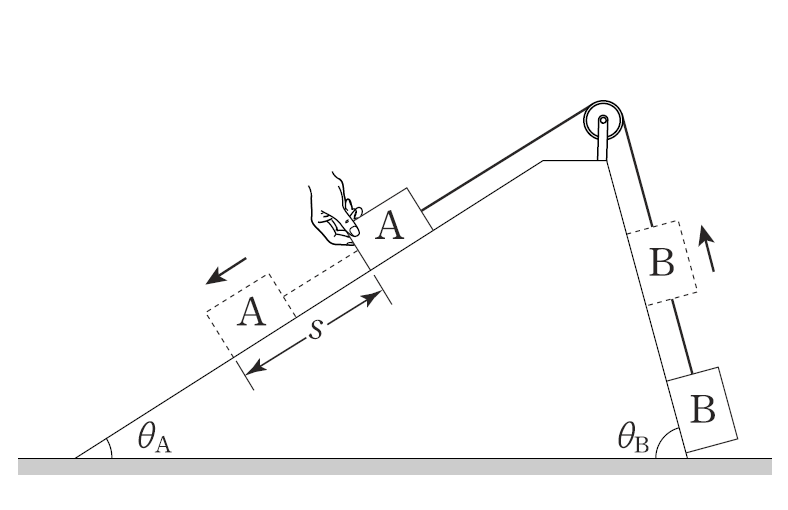
\includegraphics[scale =0.5]{180820.PNG}
    \label{fig:my_label}
\end{figure}


실을 끊은 순간부터 $B$의 변위가 0이 되었을 때, $A$의 이동거리는? (단, 모든 마찰은 무시한다.)
\ansone{4$s$}{\dfrac{13}{3}$s$}{\dfrac{14}{3}$s$}{3$s$}{\dfrac{16}{3}$s$}

\end{document}